% for slides
\documentclass{beamer}

% for 1 page per slide printouts
% \documentclass[handout]{beamer}
% \usepackage{pgfpages}
% \pgfpagesuselayout{resize to}[a4paper,landscape,border shrink=5mm]

%\documentclass[handout]{beamer}
%\usepackage{pgfpages}
%\pgfpagesuselayout{4 on 1}[a4paper,landscape,border shrink=5mm]

% \documentclass[handout]{beamer}
% \usepackage{pgfpages}
% \pgfpagesuselayout{2 on 1}[a4paper,border shrink=5mm]

\usepackage{oz}
\usepackage{multicol}
\usepackage{multimedia}
\usepackage{mathtools}

\newcommand{\Poincare}{Poincar\'{e}}
\newcommand{\Complex}{\mathbb{C}}
\newcommand{\RP}[1]{\mathfrak{R}\left(#1\right)}
\newcommand{\Real}{\mathbb{R}}
\newcommand{\Rational}{\mathbb{Q}}
\newcommand{\Integer}{\mathbb{Z}}
\newcommand{\Natural}{\mathbb{N}}
\newcommand{\CP}{\mathbf{CP}}

\newcommand{\PTIME}{\mathbf{P}}
\newcommand{\NPTIME}{\mathbf{NP}}
\newcommand{\DTIME}{\mathbf{DTIME}}
\newcommand{\NTIME}{\mathbf{NTIME}}

\renewcommand{\vec}[1]{\mathbf{#1}}

\usetheme[progressbar=title]{metropolis}           % Use metropolis theme
\title{The Millennium Prize Problems}
\subtitle{A PGR Seminar in Two Parts}
\date{}
\author{Luke Smallman}
\institute{Cardiff University} \titlegraphic{\hfill
\includegraphics[height=1.5cm]{logo}}


\begin{document}
  \maketitle
  \begin{frame}{Structure}
      \begin{multicols}{2}
          \tableofcontents
      \end{multicols}
  \end{frame}

  \section{Introduction}
  \begin{frame}{Introduction}
      \pause
      \begin{itemize}
          \item The Millennium Prize Problems were seven unsolved problems
              set out by the Clay Mathematics Institute
      \pause
          \item The Millenium Prize Problems are now six unsolved problems
              and one solved problem.
      \pause
          \item They have a certain level of infamy due to the Clay
              Mathematics Institute's promise of \$1 million for a correct
              proof of any of the problems
      \end{itemize}
  \end{frame}
  \begin{frame}{Even Elementary knows what the MPP are}
      \begin{center}
      \movie[width=\textwidth]{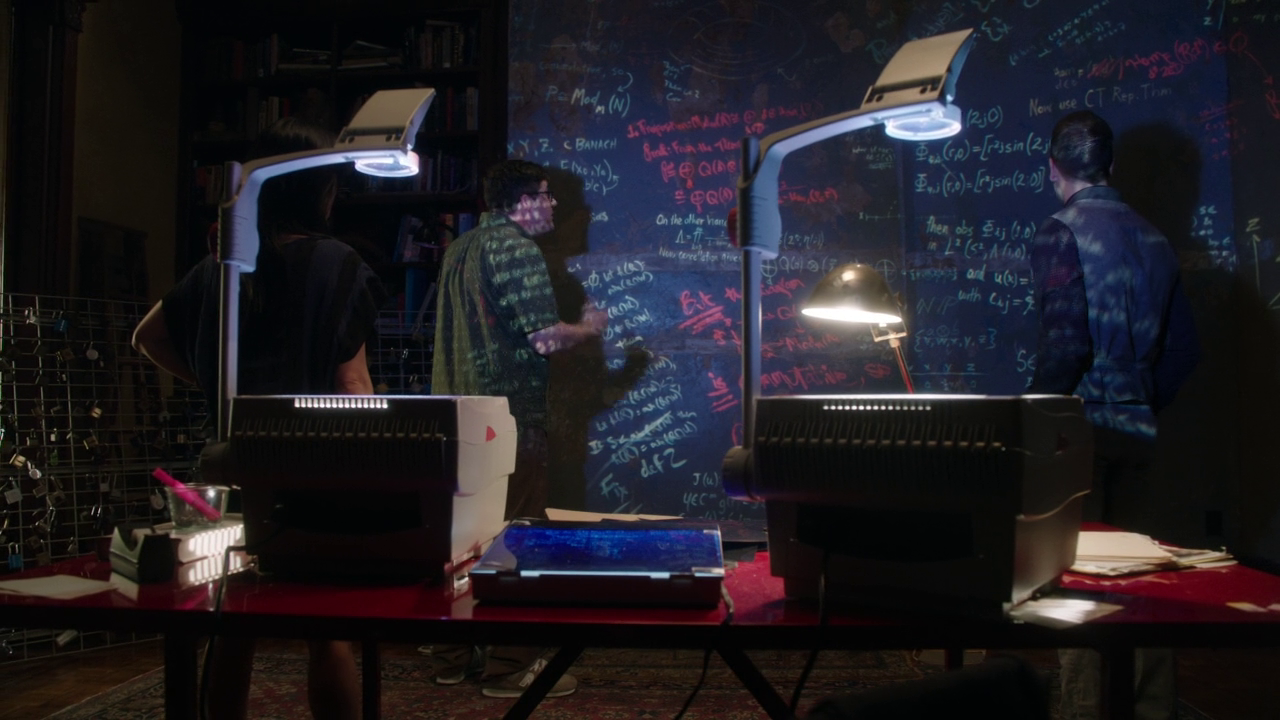
\includegraphics[width=\textwidth]{PvNPscreen.png}}{PvNP.mkv}
  \end{center}
  \end{frame}

  \section{$\PTIME$ versus $\NPTIME$}
  \begin{frame}{$\PTIME$ vs $\NPTIME$}
      \begin{block}{Problem Statement}
          Prove or disprove that $\PTIME = \NPTIME$
      \end{block}
  \end{frame}
  \subsection{What is $\PTIME$?}
  \begin{frame}{The Deterministic Turing Machine}
      \pause
      \begin{block}{Definition}
          \pause
          \begin{table}[]
              \centering
              \begin{tabular}{ll}
                  $\Box$ & The symbol denoting a blank \pause \\
                  $\Gamma \ni \Box$
                  & A finite \textit{alphabet} for the \textit{tape} \pause \\
                  $\Sigma \subseteq \Gamma \setminus \Box$ 
                  & The \textit{input} alphabet \pause \\
                  $Q$ & A finite, non-empty set of states \pause \\
                  $F \subseteq Q$
                  & The \textit{final} or \textit{accepting} states \pause \\
                  $q_0 \in Q$ & The initial state \pause \\
                  $\delta: Q \setminus F \times \Gamma \pfun Q
                  \times \Gamma \times \{L, R\}$ & The transition function
              \end{tabular}
          \end{table}
          \pause
          A DTM is then a 7-tuple
          $M = \langle Q, \Gamma, \Box, \Sigma, \delta, q_0, F \rangle$
      \end{block}
  \end{frame}
  \begin{frame}{Complexity Class $\PTIME$}
      Now we are ready to define $\PTIME$
      \pause
      \begin{block}{Definition}
          A computational problem belongs to
              $\DTIME\left(f(n)\right)$ if it can be solved by a
              DTM in $O(f(n))$ computational time 
              \pause
          $$\PTIME = \bigcup_{k \in \Natural}
              \DTIME\left(n^k\right)$$
      \end{block}
  \end{frame}
  \subsection{What is $\NPTIME$}
  \begin{frame}{The Non-Deterministic Turing Machine}
      \pause
      \begin{block}{Definition}
          \pause
          \begin{table}[]
              \centering
              \begin{tabular}{ll}
                  $\Box$ & The symbol denoting a blank \pause \\
                  $\Gamma \ni \Box$
                  & A finite \textit{alphabet} for the \textit{tape} \pause \\
                  $\Sigma \subseteq \Gamma \setminus \Box$ 
                  & The \textit{input} alphabet \pause \\
                  $Q$ & Finite, non-empty set of states \pause \\
                  $F \subseteq Q$
                  & The \textit{final} or \textit{accepting} states \pause \\
                  $q_0 \in Q$ & The initial state \pause \\
                  $\delta \subseteq (Q \setminus F \times \Gamma ) \times (Q
                  \times \Gamma \times \{L, R\})$ & The transition relation
              \end{tabular}
          \end{table}
          \pause
          An NDTM is then a 7-tuple
          $M = \langle Q, \Gamma, \Box, \Sigma, \delta, q_0, F \rangle$
      \end{block}
  \end{frame}
  \begin{frame}{Complexity Class $\NPTIME$}
      Now we are ready to define $\NPTIME$
      \pause
      \begin{block}{Definition}
          A computational problem belongs to
              $\NTIME\left(f(n)\right)$ if it can be solved by an
              NDTM in $O(f(n))$ computational time 
              \pause
          $$\NPTIME = \bigcup_{k \in \Natural}
              \NTIME\left(n^k\right)$$
      \end{block}
  \end{frame}

  \section{Riemann Hypothesis}
  \begin{frame}{Riemann Hypothesis}
      \begin{block}{Problem Statement}
          Prove that all non-trivial zeros of $\zeta(s)$ have real part
          $\frac{1}{2}$
      \end{block}
  \end{frame}
  \begin{frame}{Riemann Zeta Function}
      \pause
      \begin{block}{First definition}
          $$
          \zeta\left(s\right) = \sum_{n=1}^{\infty} \frac{1}{n^s} \qquad
          s \in (1, \infty)
          $$
      \end{block}
      \pause
      \centering
      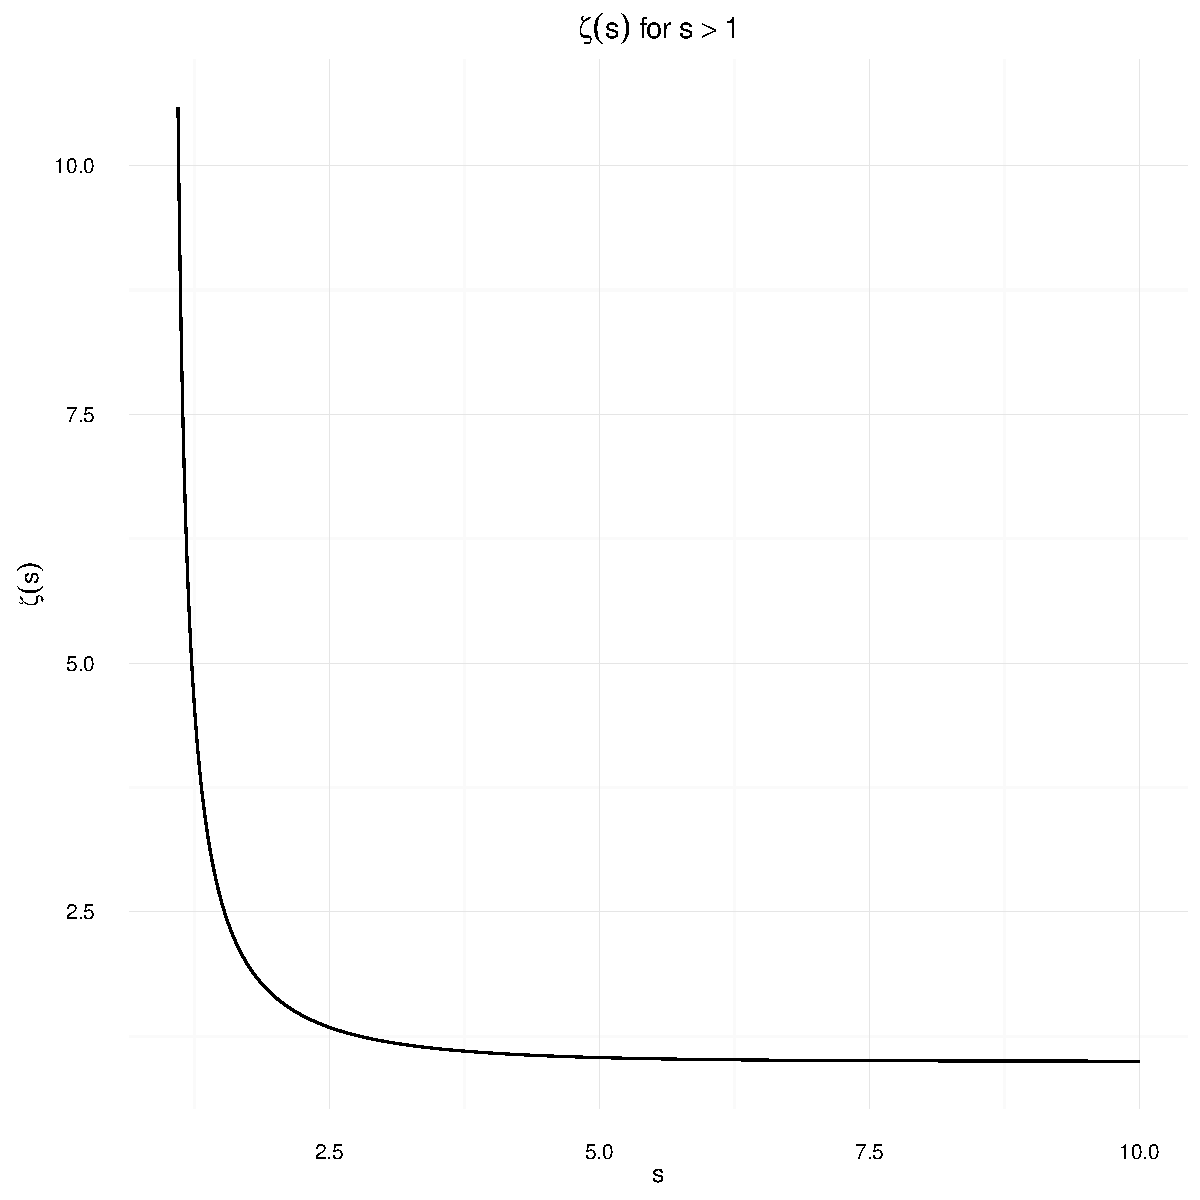
\includegraphics[width=0.5\textwidth]{zetagreater1.pdf}
  \end{frame}
  \begin{frame}{Riemann Zeta Function}
      \pause
      \begin{block}{Second definition}
          $$
          \zeta\left(s\right) = \sum_{n=1}^{\infty} \frac{1}{n^s} \qquad
          s \in \Complex; \RP{s} > 1
          $$
      \end{block}
      \pause
      \begin{block}{Third Definition}
          $\zeta(s)$ is the (unique) analytic continuation of the function in
          the second definition for all $s \ne 1$
      \end{block}
  \end{frame}
  \begin{frame}{Riemann Zeta Function}
      \pause
      \begin{block}{Fourth Definition}
          $$
          \zeta\left(s\right) = \product_{p \textrm{ prime}} \frac{1}{1 - p^{-s}}
          $$
      \end{block}
  \end{frame}
  \begin{frame}{Zeros}
      \pause
      \begin{block}{Trivial Zeros}
          $$
          \zeta(s) = 0 \quad \forall s \in \left\{-2, -4, -6, \ldots \right\}
          $$
      \end{block}
      \pause
      \begin{block}{Non-Trivial Zeros}
          So far, every non-trivial zero of $\zeta(s)$ which has been found
          lies on the line $\frac{1}{2} + it, t \in (-\infty, \infty)$.
      \end{block}
      \pause
      \begin{block}{Highly Non-Trivial Zeros}
          The statement of the problem is concerned with the existence of
          non-trivial zeros which do not lie on that line.
      \end{block}
  \end{frame}
  \begin{frame}{Consequences of the Riemann Hypothesis}
      \pause
      \begin{block}{Prime Number Theorem}
          Using RH we get a tight bound on the remainder term of the prime
          number theorem expression for the number of primes below $x$
          $$
          \pi(x) = \underbrace{\integral_{2}^{x} \frac{1}{\log t}
          dt}_{\eqqcolon Li(x)} + O(\sqrt{x}\log x)
          $$\pause
          In particular, RH implies
          $$
          \left| \pi(x) - Li(x) \right| < \frac{1}{8\pi}\sqrt{x}\log x \quad
          x \ge 2657
          $$
      \end{block}
  \end{frame}
  \begin{frame}{Consequences of the Riemann Hypothesis}
      \pause
      \begin{block}{Growth of the Divisor Function}
          Let $\sigma(n) = \sum_{d | n}d$. Then RH implies
          $$
          \sigma(n) < e^{\gamma} n \log\log n \quad n > 5040
          $$
      \end{block}
  \end{frame}

  \section{Navier-Stokes Existence and Smoothness}
  \subsection{Problem Statement}
  \begin{frame}{Navier-Stokes Existence and Smoothness}
      \begin{block}{Problem Statement}
          Prove that there exist smooth solutions with finite energy of the
          Navier-Stokes equations for any given divergence-free initial
          velocity field with no external force applied on either $\Real^3$
          or $\Real^3/\Integer$.\pause\\
          OR prove that there exists a divergence-free
          intial velocity field and a smooth external force which does not
          have a smooth solution with finite energy.
      \end{block}
  \end{frame}
  \subsection{Navier-Stokes Equations}
  \begin{frame}{Navier-Stokes Equations}
      \pause
      \begin{block}{Material Derivative}
          We define $\frac{D}{Dt} \coloneqq \frac{\partial}{\partial t} +
          \mathbf{u} \cdot \nabla$
      \end{block}
      \pause
      \begin{block}{Incompressible Navier-Stokes}
          $$
          \frac{D \mathbf{u}}{D t} = -\nabla p + \nu\nabla^2\mathbf{u} +
          \mathbf{F}
          $$\pause
          $$
          \nabla \cdot \mathbf{u} = 0
          $$
      \end{block}
      \pause
      \begin{block}{Initial Conditions}
          $$
          \mathbf{u}(\mathbf{x}, 0) = \mathbf{u}^0(\mathbf{x}), \quad
          \mathbf{u}^0 \in C^{\infty},\; \nabla \cdot \mathbf{u}^0 = 0
          $$
      \end{block}
  \end{frame}
  \begin{frame}{Conditions Imposed}
      \linespread{0.8}
      \pause
      \begin{block}{Conditions Imposed on $\mathbf{u}^0$ and $\mathbf{F}$}
          We require:
          $$
          \left| \partial^{\boldsymbol{\alpha}}_{\mathbf{x}} \mathbf{u}^0
          \right| \le
          C_{\boldsymbol{\alpha}K} \left(1 + \left|\mathbf{x}\right|\right)^{-K} \quad
          \forall K > 0, \; \forall \boldsymbol{\alpha} \in \Natural_0^3, \;
          \forall \mathbf{x} \in \Real^3
          $$\pause
          \begin{multline*}
          \left| \partial^{\boldsymbol{\alpha}}_{\mathbf{x}}
          \partial^m_t \mathbf{F}
          \right| \le
          C_{\boldsymbol{\alpha}mK} \left(1 + \left|\mathbf{x}\right| +
          t\right)^{-K} \\
          \forall K > 0, \; \forall \boldsymbol{\alpha} \in \Natural_0^3, \;
          \forall m \in \Natural_0, \; \forall \mathbf{x} \in \Real^3, \;
          \forall t \in [0, \infty)
          \end{multline*}
      \end{block}
      \pause
      \begin{block}{Physically Reasonable Solutions}
          We require
          $$
          p, \mathbf{u} \in C^{\infty}(\Real^3 \times [0, \infty))
          $$
          \pause
          $$
          \integral_{\Real^n} \left| \mathbf{u}(\mathbf{x}, t) \right|^2
          d\mathbf{x} < C \quad \forall t \in [0, \infty)
          $$
      \end{block}
  \end{frame}
  \begin{frame}{Navier-Stokes Existence and Smoothness}
      \begin{block}{Problem Statement}
          Prove that there exist smooth solutions with finite energy of the
          Navier-Stokes equations for any given divergence-free initial
          velocity field with no external force applied on either $\Real^3$
          or $\Real^3/\Integer$.\pause\\
          OR prove that there exists a divergence-free
          intial velocity field and a smooth external force which does not
          have a smooth solution with finite energy.
      \end{block}
  \end{frame}

  \section{\Poincare{} Conjecture}
  \subsection{Problem Statement}
  \begin{frame}{\Poincare{} Conjecture}
      \begin{block}{Problem Statement}
          Prove that every simply connected, closed 3-manifold is
          homeomorphic to the 3-sphere.
      \end{block}
  \end{frame}
  \subsection{Topology and Manifolds}
  \begin{frame}{Manifolds}
      \linespread{0.9}
      \pause
      \begin{block}{Topology}
          Given a set $X$, a \textit{topology} $\tau$ on $X$ is a collection of
          subsets of $X$ such that
          \begin{itemize}
              \item $X \in \tau, \emptyset \in \tau$
              \item The union of any collection of elements of $\tau$ is in
                  $\tau$
              \item The intersection of any \alert{finite} collection of
                  elements of $\tau$ is in $\tau$
          \end{itemize}
          The elements of $\tau$ are then called \textit{open sets}
      \end{block}
      \pause
      \begin{block}{Topological Field}
          A \textit{topological field} is a field which is also endowed with a
          topology.
      \end{block}
      \pause
      \begin{block}{Topological Vector Space}
          A \texit{topological vector space} is a vector space $X$ over a
          topological field $\mathbf{K}$ which is endowed with a topology such
          that vector addition and scalar multiplication are continuous
          functions.
      \end{block}
  \end{frame}
  \begin{frame}{Manifolds}
      \linespread{0.8}
      \pause
      \begin{block}{Homeomorphism}
          A \textit{homeomorphism} is a continuous function between two
          topological spaces whose inverse is continuous.
      \end{block}
      \pause
      \begin{block}{Manifolds}
          A \textit{manifold} $M$ is a topological space which is locally
          homeomorphic to a topological vector space.
      \end{block}
      \pause
      \begin{block}{Compact Manifold}
          A manifold $M$ is \textit{compact} if for every open cover there
          exists a finite subcover. That is
          \begin{multline*}
              \linespread{0.8}
          \forall \left\{U_a\right\}_{a \in A} \textrm{ s.t } \bigcup_{a\in A}
          U_a = M,
          U_a \textrm{ open}\\
          \exists J \subset A, |J| < \infty : \bigcup_{j \in J}U_j = M
          \end{multline*}
      \end{block}
  \end{frame}
  \begin{frame}{Manifolds}
      \linespread{0.8}
      \pause
      \begin{block}{Closed Manifold}
          A manifold is \textit{closed} if it is compact and does not contain
          its boundary
      \end{block}
      \pause
      \begin{block}{Path Connected}
          A manifold $M$ is \textit{path connected} if there exists a path
          connecting every two points in $M$
      \end{block}
      \pause
      \begin{block}{Simply Connected}
          Formally, a manifold $M$ is \textit{simply connected} if it is path
          connected and any two paths from $x \in M$ to $y \in M$ are
          homotopic relative to their endpoints
      \end{block}
      \pause
      \begin{block}{3-Manifold}
          A \textit{3-manifold} is a manifold which is locally homeomorphic to
          $\Real^3$
      \end{block}
      \pause
      \begin{block}{3-Sphere}
          $S^3 = \left\{\left(x_0, x_1, x_2, x_3) \in \Real^4 | x_0^2 + x_1^2 + x_2^2 +
          x_3^2 = 1\right\}$
      \end{block}
  \end{frame}
  \begin{frame}{\Poincare{} Conjecture}
      \begin{block}{Problem Statement}
          Prove that every simply connected, closed 3-manifold is
          homeomorphic to the 3-sphere.
      \end{block}
  \end{frame}

  \section{Pause}
  \begin{frame}{Questions}
      \begin{block}{}
          Any questions?
      \end{block}
  \end{frame}


  \section{Hodge Conjecture}
  \begin{frame}{Hodge Conjecture}
      \begin{block}{Problem Statement}
          Prove that on a projective non-singular algebraic variety over
          $\Complex$, any Hodge class is a rational linear combination of
          classes $cl(Z)$ of algebraic cycles.
          \note{This definition comes from the CMI}
      \end{block}
      % \begin{block}{Problem Statement}
      %     Let $X$ be a non-singular complex projective manifold. Then every
      %     Hodge class on $X$ is a linear combination with rational
      %     coefficients of the cohomology classes of complex subvarities of $X$.
      %     \note{This definition comes from wikipedia}
      % \end{block}
  \end{frame}
  \begin{frame}{Projective Algebraic Varieties over $\Complex$}
      \pause
      \begin{block}{Complex Projective Space}
          The \textit{complex projective space} of dimension $n$, denoted by
          $\CP^n$, is the set of all \alert{complex} lines in $\Complex^{n+1}$
          which pass through the origin.
      \end{block}
      \pause
      \begin{block}{Homogeneous Coordinates}
          We can identify each line in a complex projective space with a set of
          \textit{homogeneous coordinates}, usually denoted $[z_1 : z_2 :
          \cdots : z_{n+1}]$. These are unique up to scalar multiplication.
      \end{block}
      \pause
      \begin{block}{Homogeneous Polynomial}
          A \textit{homogeneous polynomial} is a polynomial whose non-zero
          terms have the same degree.
          \pause\\
          Important property: if $P(\vec{x})$ is homogeneous, then
          $$P(\lambda\vec{x}) = \lambda^d P(\vec{x})$$
      \end{block}
  \end{frame}

  % \begin{frame}{Complex Manifolds}
  %     \pause
  %     \begin{block}{Topological Field}
  %         A \textit{topological field} is a field which is also endowed with a
  %         topology.
  %     \end{block}
  %     \pause
  %     \begin{block}{Topological Vector Space}
  %         A \texit{topological vector space} is a vector space $X$ over a
  %         topological field $\mathbf{K}$ which is endowed with a topology such
  %         that vector addition and scalar multiplication are continuous
  %         functions.
  %     \end{block}
  %     \pause
  %     \begin{block}{Manifolds}
  %         A \textit{manifold} $M$ is a topological space which is locally
  %         homeomorphic to a topological vector space.
  %     \end{block}
  % \end{frame}
  % \begin{frame}{Complex Manifolds 2}
  %     \pause
  %     \begin{block}{Charts and Atlases}
  %         A \textit{chart} is an ordered pair $(U, \phi)$, where $U \subset M$
  %         is open and $\phi$ is a homeomorphism from $U$ to a topological
  %         vector space. \pause \\
  %         An \textit{atlas} is a collection of charts $(U_i, \phi_i)$ such that
  %         $\bigcup_i U_i = M$. \pause
  %     \end{block}
  %     \begin{block}{Complex Manifolds}
  %         A \textit{complex manifold} is a manifold whose atlas of charts
  %         gives homeomorphisms into the open unit disk in $\Complex^n$.
  %     \end{block}
  % \end{frame}
  % \begin{frame}{Complex Projective Manifolds}
  %     \pause
  %     \begin{block}{Embeddings}
  %         An \textit{embedding} is a homeomorphism onto its image. That is,
  %         $f: X \hookrightarrow Y$ is an embedding if it is injective,
  %         continuous, and forms a homeomorphism from $X$ to $f(X)$, with 
  %         $f(X)$ inheriting the subspace topology of $Y$.
  %     \end{block}
  %     \pause
  %     \begin{block}{Complex Projective Space}
  %         The \textit{complex projective space} of dimension $n$, denoted by
  %         $\CP^n$, is the set of all \alert{complex} lines in $\Complex^{n+1}$
  %         which pass through the origin.
  %     \end{block}
  %     \pause
  %     \begin{block}{Complex Projective Manifold}
  %         A \textit{complex projective manifold} is a complex manifold which
  %         can be embedded in complex projective space.
  %     \end{block}
  % \end{frame}
  % 

  \section{Yang-Mills Existence and Mass Gap}
  \begin{frame}{Yang-Mills Existence and Mass Gap}
      \begin{block}{Problem Statement}
          Prove that for any compact simple gauge group $G$, a non-trivial
          quantum Yang-Mills theory exists on $\Real^4$ and has a mass gap
          $\Delta > 0$.
      \end{block}
  \end{frame}

  \section{Birch and Swinnerton-Dyer Conjecture}
  \begin{frame}{Birch and Swinnerton-Dyer Conjecture}
      \begin{block}{Problem Statement}
          Prove that the Taylor expansion at $s=1$ of the incomplete
          $L$-function $L(C, s)$ of non-singular projective model $C$ of a
          curve $C_0$ defined by $f(x, y) = 0$ for a polynomial
          $f \in \Rational [x, y]$ has the form
          $c(s-1)^r + \text{higher order terms}$ with
          $r = \mathrm{rank}(C(\Rational))$.
      \end{block}
  \end{frame}



\end{document}
